\documentclass[../thesis/thesis.tex]{subfiles}
\begin{document}

\chapter{Evaluation}
\label{chap:evaluation}

We believe it is possible to produce an improved \gls{vc} investment screening system. In Chapter~\ref{chap:design}, we described the design and development of such a system. Our system identifies startup companies likely to receive additional funding or exit in a given forecast window. In this chapter, we perform a series of experiments to evaluate our system against criteria of practicality, robustness and versatility.

\begin{enumerate}

\item Practicality. We designed our system to require minimal user input. Therefore, by virtue of its design, the proposed system is more efficient than current systems. We also explored the time profile of our system. An indicative implementation of our system takes 46 hours to run.

\item Robustness. We observed minimal variance in the performance and types of models generated by our system across training sets of various dates. We also evaluated the learning curves of our system and identified that our system is likely to adapt and perform better as the data sources grow over time.

\item Versatility. We assessed our system's ability to perform a variety of investment prediction tasks. Tasks included predicting companies at different developmental stages, for different target outcomes, and over different forecast windows. Our system performs best for longer forecast windows (up to 4 years) and companies at later developmental stages (e.g. Series B, C).

\end{enumerate}

\section{Experimental Design}

In this chapter, we evaluate models generated by our system while varying a number of other factors. This evaluation process is depicted in Figure~\ref{fig:evaluation:pipeline_evaluation}. The optimised pipeline is fit to a training dataset to generate a model. The model is applied to a test feature vector to produce predictions. We scored these predictions against truth values derived from a held-out test database collected in April 2017. This process is performed multiple times to evaluate the system against the three criteria derived from our literature review: practicality, robustness and versatility. The configuration of the system during our experiments is detailed in Appendix~\ref{appendix:experimental_config}.

\begin{figure}[!htb]
    \centering
    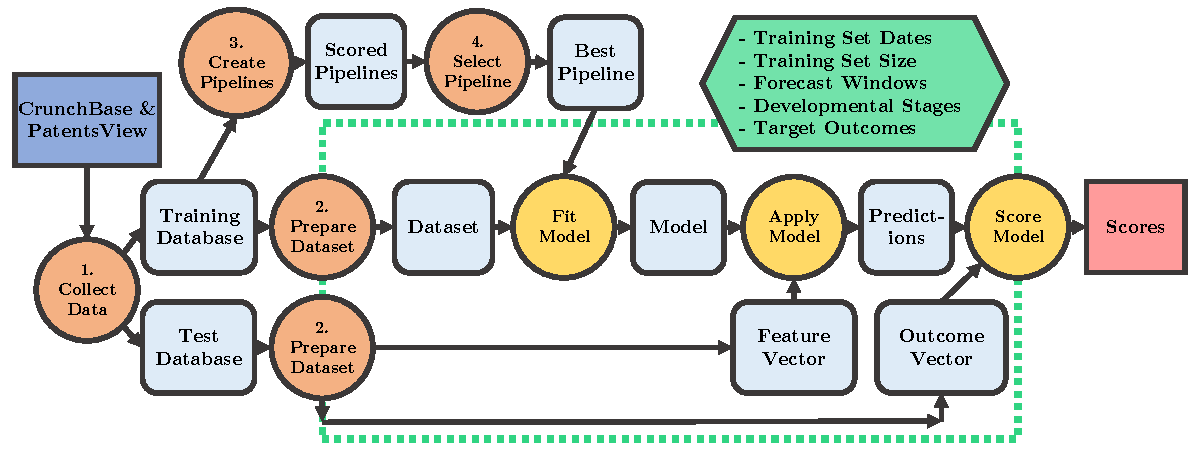
\includegraphics[width=\textwidth]{../figures/evaluation/flowchart_evaluation}
    \caption[Pipeline evaluation flowchart]{Pipeline evaluation overview. Training and test datasets are generated according to the experimental configuration: varying with respect to training set dates, training set size, forecast window, developmental stage, and target outcomes. Legend: dark blue square~=~input, orange circle~=~system component, yellow circle~=~process, light blue rounded square~=~intermediate, red square~=~output, green hexagon: iterative process / search space.}
    \label{fig:evaluation:pipeline_evaluation}
\end{figure}

\subsection{Baseline Analysis}

Before we evaluated our system, we performed preliminary analyses to determine the baseline trends and distributions of company outcomes in our database.

First, we explored company outcomes by forecast window. We applied the same system of reverse-engineering time slices that we used in previous experiments on robustness, but this time we varied the time passed between our feature vector and outcome vector (i.e. the forecast window). We created datasets from feature and outcome vectors of each year from 2012-2016 and explored the proportion of companies that raised additional funding, were acquired or had an \gls{ipo}.

Figure~\ref{fig:evaluation:outcome_forecast_window} shows how company outcome varies with respect to the forecast window (time between the observed features and the measured outcome). We observe a positive relationship between length of forecast window and company outcome. For additional funding rounds, this relationship disappears after three years. This finding implies that companies that do not raise additional funding rounds over a three year period are unlikely to raise further funds at all. We do not observe this effect for acquisitions or IPOs which implies there is either greater variability in the time it takes companies to exit or the lead-time to exit for most companies in our dataset is longer than four years. Few companies exited (1.2\%) or raised funds (5\%)over a period of fewer than two years which suggests we should focus our experimentation on forecast windows of 2--4 years.

\begin{figure}[!htb]
    \centering
    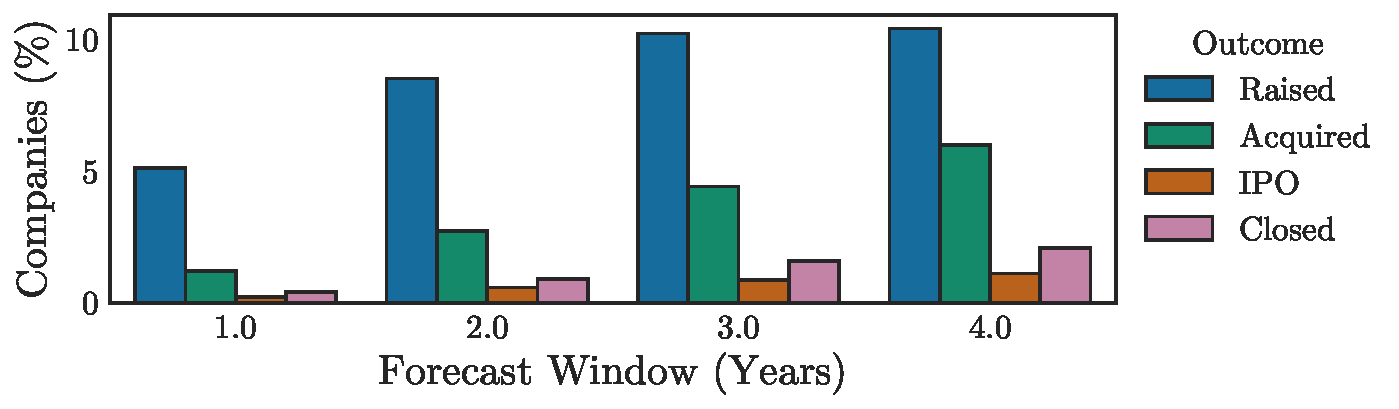
\includegraphics[width=\textwidth]{../figures/evaluation/outcomes_window}
    \caption[Outcomes by forecast window]{Outcomes by forecast window.}
    \label{fig:evaluation:outcome_forecast_window}
\end{figure}

We also explored how company outcomes vary with respect to development stage, shown in Figure~\ref{fig:evaluation:outcome_stage}. We see a broad positive relationship between developmental stage and likelihood of further funding rounds and exits. There is a high proportion of later stage companies in our dataset that do not receive additional funding or exit over four years. Only a small proportion of companies in our dataset are reported to be Closed. We can guess that many companies that do not raise or exit may have closed or down-sized. We also observe considerable variation in the outcomes of companies of different developmental stages. For example, only a small proportion of companies perform an \gls{ipo} before Series C stage. We decided to investigate how our system predicts outcomes for each developmental stage independently, as well as in aggregate.

\begin{figure}[!htb]
    \centering
    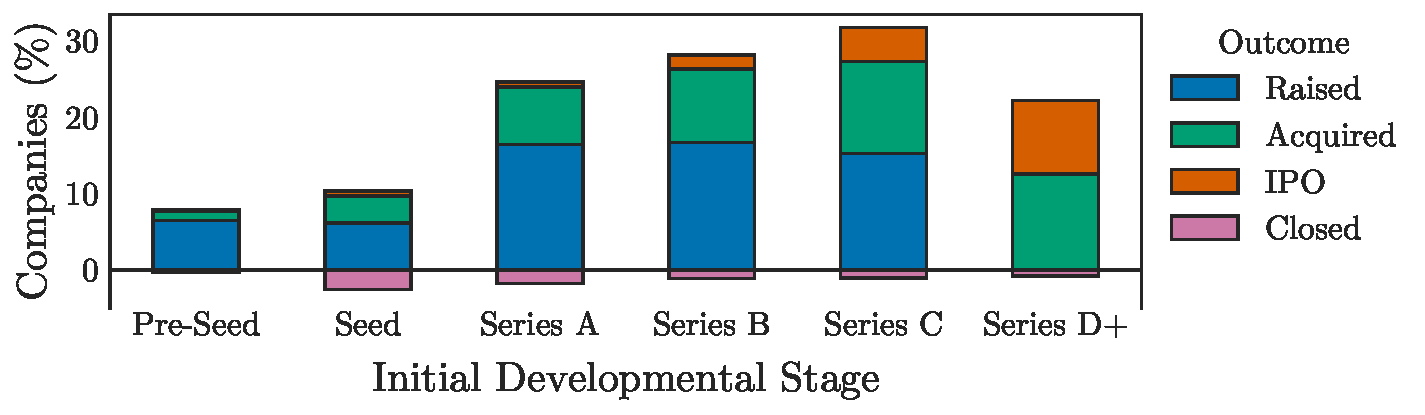
\includegraphics[width=\textwidth]{../figures/evaluation/outcomes_stage}
    \caption[Outcomes by developmental stage]{Outcomes by developmental stage.}
    \label{fig:evaluation:outcome_stage}
\end{figure}

\subsection{Evaluation Metrics}

While Area under the \gls{pr} Curve was used to guide the development of our system, in evaluation of our system's performance we primarily use F1 Scores. An F1 score is the harmonic mean of recall and precision at points on the \gls{pr} curve. The harmonic mean is an alternative to the arithmetic mean that tends strongly towards the smallest element in a set. Accordingly, F1 Scores are highly sensitive to trade-offs between recall and precision. The \gls{auc} measure provides an overall evaluation of a classification system, whereas the F1 Score evaluates a set of predictions. For investment screening, we are more sensitive to classification performance for the positive class (companies that have been successful in raising further funding or achieving an exit), so hereafter, when we refer to F1 Score, we refer to the F1 Score for this class alone. We also present \gls{mcc} in some of our analyses. \Gls{mcc} is a measure of the correlation between the observed and predicted binary classifications. The \gls{mcc} should produce similar results to an F1 Score that incorporates performance across both positive and negative classes.

\section{Practicality}

The \gls{vc} industry requires more efficient forms of investment analysis, particularly in surfacing and screening. \Gls{vc} firms currently perform these processes through referral, Google search, industry papers and manual search of startup databases. Our automated system is more efficient than these methods because it is designed to involve minimal user input. However, it is also important that our system is relatively time-efficient so that it can run frequently enough so that its predictions are always up-to-date and relevant. We assess the time profile of our system to determine whether it is practical for use in the \gls{vc} industry.

An indicative time profile of the system is shown in Table~\ref{tab:evaluation:time_profile}. At the highest-level, this configuration of the program takes 46 hours to complete on a modern desktop PC. When we further break this time down by system component, the vast majority of time (84.8\%) is taken up by the initial pipeline creation component. This time is due to the pipeline optimisation process -- the model is fit and scored over 500 times on different classification algorithms and parameters. Scoring takes a long time because, in this case, it also involves generating learning curves for reporting, which is another cross-validated process. In practice, we could reduce the running time of our system by removing logging and reporting processes and by scheduling components of the system to run independently. For example, the pipeline creation process takes a long time but is relatively robust to dataset changes in the short-term, so the system could potentially run this component on a more infrequent basis.

\begin{table}[!htb]
    \centering
    \scalebox{0.9}{\newcommand{\sub}[1]{\hspace{1em}#1}

\begin{tabular}{lrrrrr} \toprule
Function & Cycle (s) & Cycles (N) & Time (s)   & Time (m) & Time (h) \\ \midrule
Generate Dataset (CV)             & 1,800 & 1 & 1,800 & 30 & 0.5 \\
\sub{Prepare Feature Dataset}     & 1,200 & 1 & 1,200 & 20 & 0.3 \\
\sub{Prepare Outcome Dataset}     & 180 & 1 & 180 & 3 & 0.1 \\
\sub{Merge Datasets}              & 360 & 1 & 360 & 6 & 0.1 \\
\sub{Finalise Dataset}            & 60 & 1 & 60 & 1 & 0.0 \\
Fit and Score Model\textsuperscript{1} & 265 & 525 & 139,125 & 2,319 & 38.6 \\
\sub{Fit Model}                   & 15 & 525 & 7,875 & 131 & 2.2 \\
\sub{Score Model}                 & 250 & 525 & 131,250 & 2,188 & 36.5 \\ \midrule
\multicolumn{3}{l}{Subtotal: Create Pipelines} & 140,925 & 2,349 & 39.1 \\ \midrule
Get Finalist Pipelines            & 5 & 1 & 5 & 0 & 0.0 \\
Generate Dataset (CV)             & 1,800 & 5 & 1,800 & 30 & 0.5 \\
Fit and Score Model\textsuperscript{2} & 265 & 75 & 19,875 & 331 & 5.5 \\
Select Best Pipeline              & 5 & 1 & 5 & 0 & 0.0 \\ \midrule
\multicolumn{3}{l}{Subtotal: Select Best Pipeline} & 21,685 & 361 & 6.0 \\ \midrule
Generate Dataset (Training)       & 1,800 & 1 & 1,800 & 30 & 0.5 \\
Generate Dataset (Test)           & 1,800 & 1 & 1,800 & 30 & 0.5 \\
Fit Model                         & 30 & 1 & 30 & 1 & 0.0 \\
Make Predictions                  & 5 & 1 & 5 & 0 & 0.0 \\ \midrule
\multicolumn{3}{l}{Subtotal: Fit and Make Predictions} & 3,635 & 61 & 1.0 \\ \midrule
\multicolumn{3}{l}{Total}        & 166,245 & 2,771 & 46.2 \\
\bottomrule \end{tabular}
}
    \caption[System time profile]{System time profile.  All times are indicative based on averages from system logs. Notes: \textsuperscript{1} Cycles involve 25 search iterations, 3 cross-validated folds, and 7 classification algorithms. \textsuperscript{2} Cycles involve 5 finalist pipelines, 3 database slices, 3 cross-validated folds.}
    \label{tab:evaluation:time_profile}
\end{table}

\section{Robustness}

An improved \gls{vc} investment screening system must be robust to changes over time. \Gls{vc} firms have concerns that models trained on historical data will not predict future trends and activity. These concerns are a key barrier to the adoption of automated systems by the \gls{vc} industry~\cite{stone2014}. Therefore, it is critical that our system is shown to be robust in its performance with respect to time so investors can rely on its predictions. Similarly, \gls{vc} firms seek systems that are themselves robust to time and can adapt to new data sources and feature sets as they become available. In the following section, we evaluate our system based on its robustness to training set dates and training set sizes.

\subsection{Training Set Date}

A \gls{vc} investment screening system should have minimal variance in its performance when training on datasets from different dates so investors can trust its ability to make future-looking predictions.

Figure~\ref{fig:evaluation:performance_slice} shows models trained on training sets sliced from various years and scored against key evaluation metrics. We held the forecast window constant at two years because we cannot test training sets from later years using long forecast windows, and this would skew our results. Variance across all evaluation metrics is low, with a slight improvement in performance for newer dataset slices which probably reflects that newer datasets provide more training data.

We explored the feature weights for each model in Figure~\ref{fig:evaluation:features_slice}. While there are some slight differences with respect to Executives, Investors, and Economic factors, the baseline distribution trend is similar across all training set dates. We discuss the distribution of these feature weights in more detail in a following section.

\begin{figure}[!htb]
    \centering
    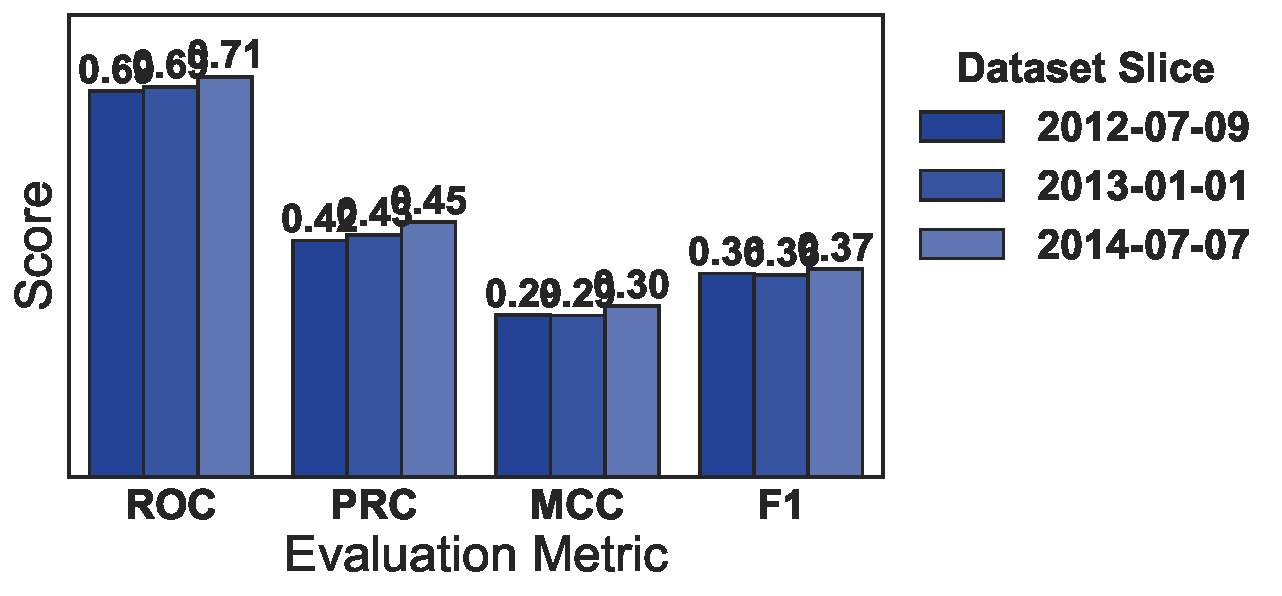
\includegraphics[width=\textwidth]{../figures/evaluation/performance_slice}
    \caption[Performance by training set date]{Performance by training set date.}
    \label{fig:evaluation:performance_slice}
\end{figure}

\begin{figure}[!htb]
    \centering
    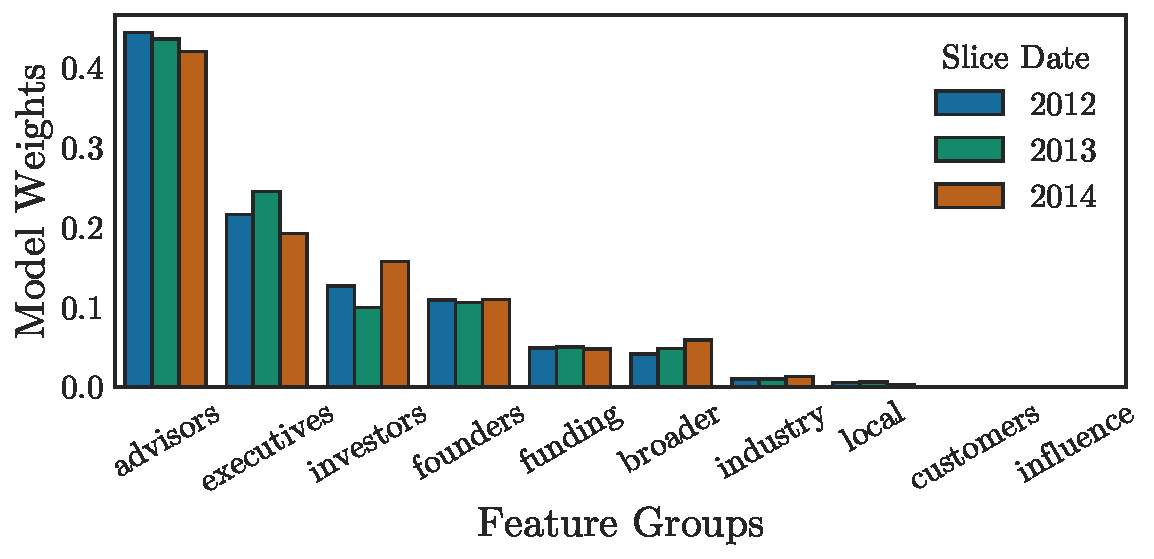
\includegraphics[width=\textwidth]{../figures/evaluation/features_slice}
    \caption[Feature weights by training set date]{Feature weights by training set date.}
    \label{fig:evaluation:features_slice}
\end{figure}

\subsection{Training Set Size}

Learning curves allow us to evaluate how the bias and variance of a classification technique vary with respect to the amount of training data available. We investigated learning curves for our system to determine whether our system's performance has potential to improve as its data sources grow. We sampled our training sets five times at different fractional rates. The rate of convergence (or divergence) of our training and cross-validation curves can indicate whether our classification pipeline is over- or under-fitting our data for various sizes. We investigated these learning curves with respect to forecast window, target outcome and developmental stage.

Figure~\ref{fig:evaluation:learning_window} shows the learning curves for forecast windows of 2--4 years against a combined target outcome and companies from all developmental stages. The maximum number of training examples is negatively related to the length of the forecast window because newer datasets have more examples. For a forecast window of four years, the curves have converged, whereas for shorter forecast windows there still seems to be some benefit to additional training examples. Much of the testing score improvement comes in the first 20,000 training examples, which suggests this pipeline is approaching optimal performance.

\begin{figure}[!htb]
    \centering
    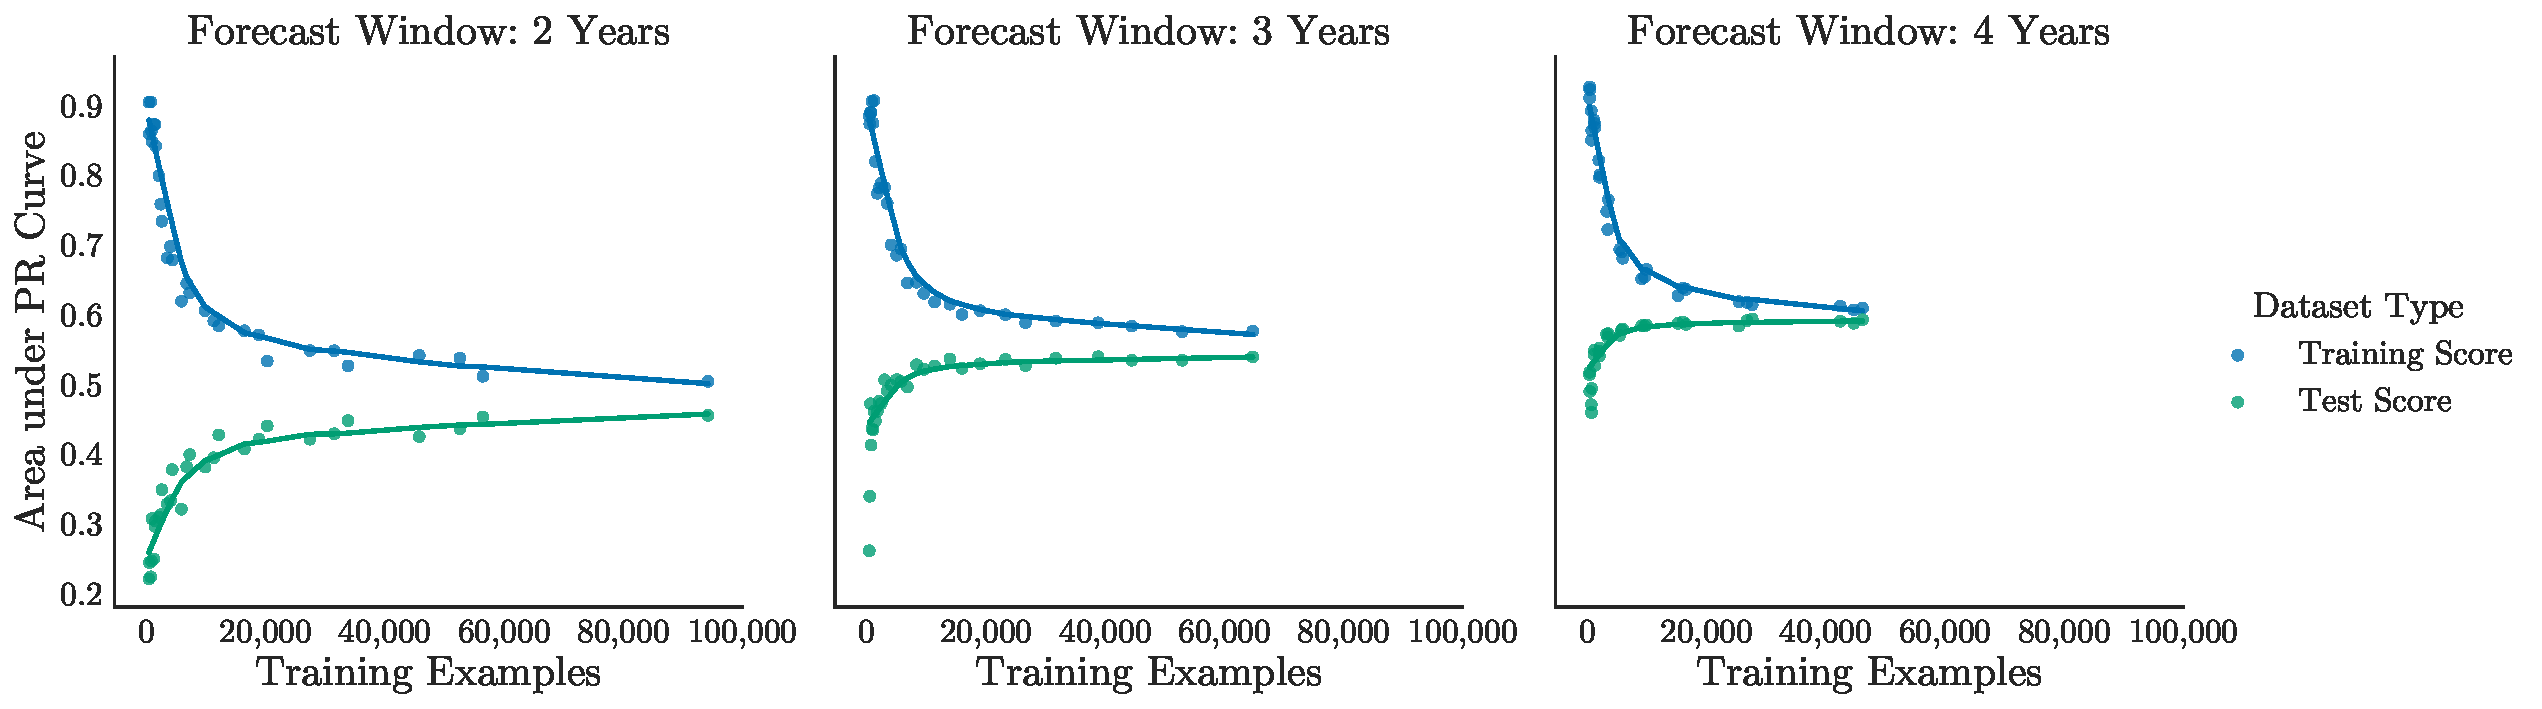
\includegraphics[width=\textwidth]{../figures/evaluation/learning_curves_window}
    \caption[Learning curves by forecast window]{Learning curves by forecast window.}
    \label{fig:evaluation:learning_window}
\end{figure}

We can measure investment success by various target outcomes. We have evaluated previous learning curve plots against a combined outcome of either raising funds, being acquired or having an \gls{ipo}. We termed this ``Extra Stage''. We see that the efficiency of our system varies with respect to these outcomes in Figure~\ref{fig:evaluation:learning_outcome_window}. Predicting whether a company raises an extra round is the least data-intensive outcome, as it converges quickly. In comparison, the plot for predicting company exits does not converge. Our model has most difficulty predicting IPOs, probably because these are rare events in our dataset.

\begin{figure}[!htb]
    \centering
    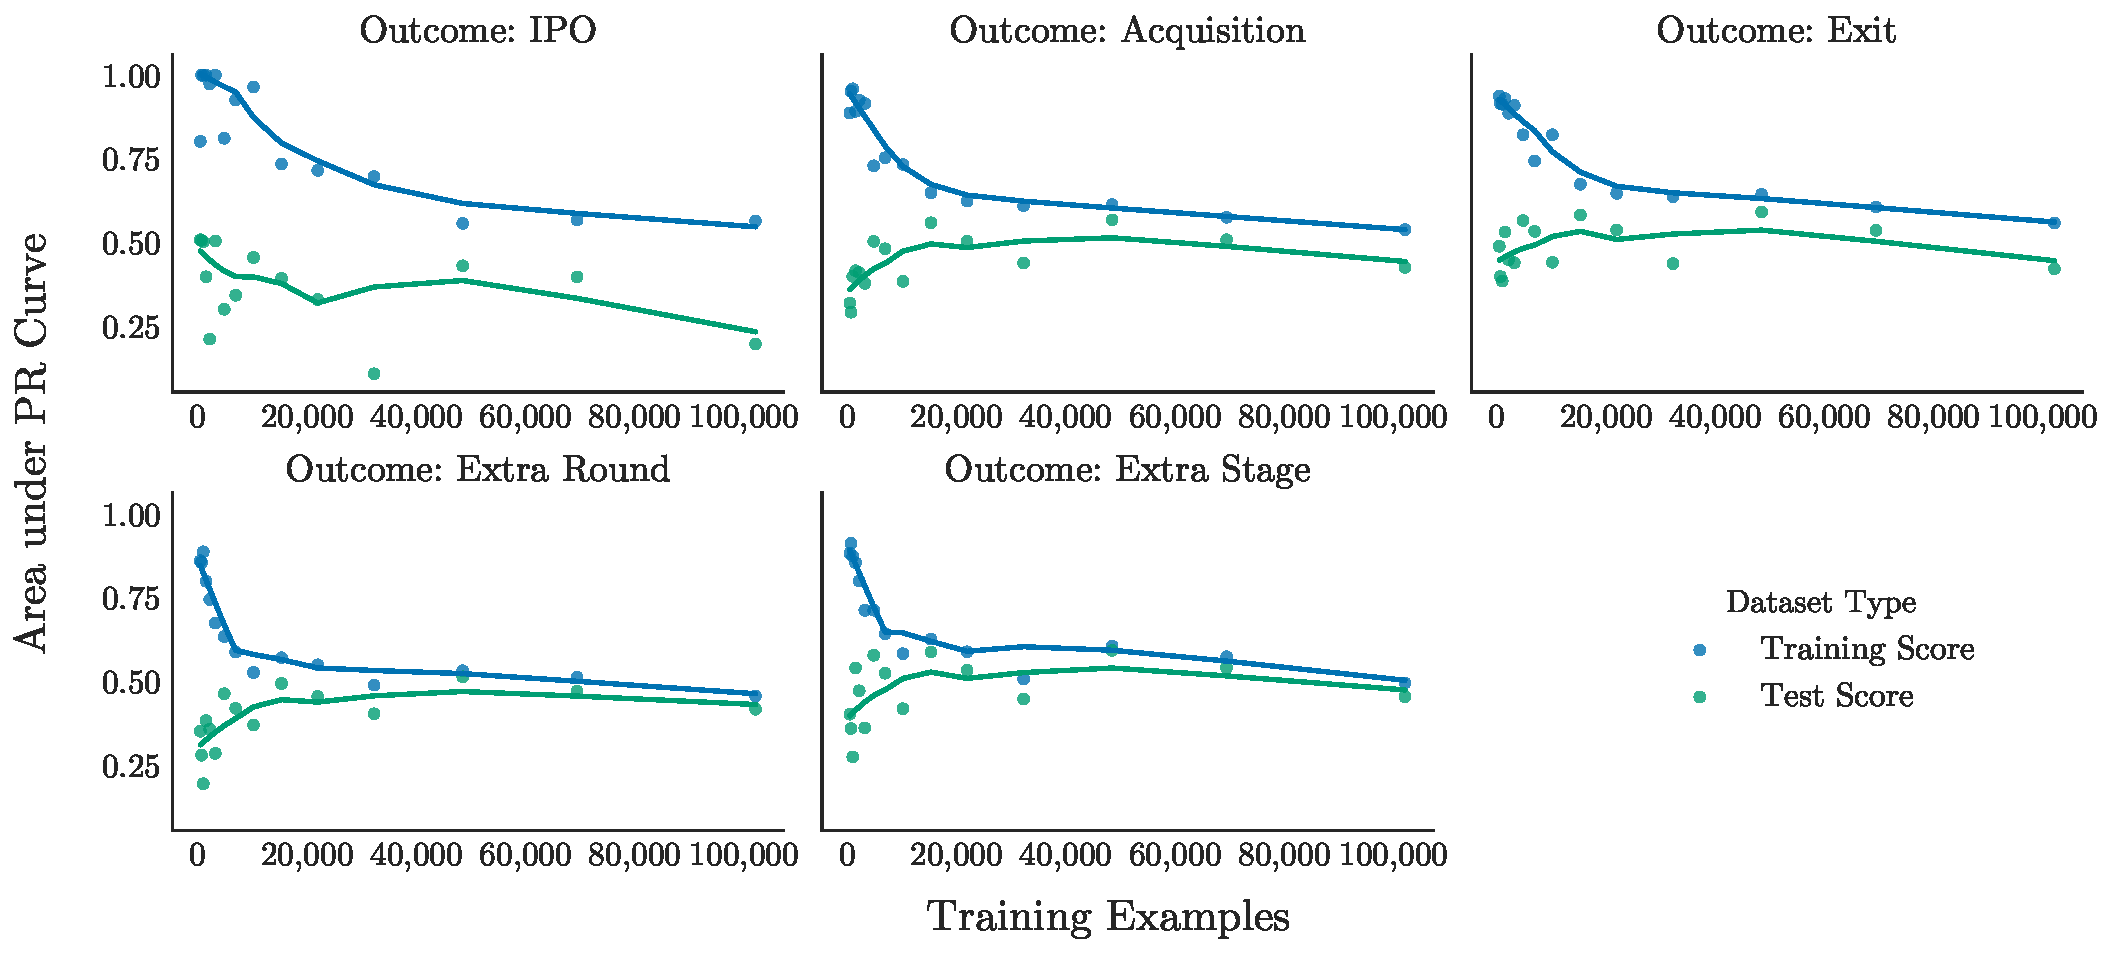
\includegraphics[width=\textwidth]{../figures/evaluation/learning_curves_outcome}
    \caption[Learning curves by target outcome]{Learning curves by target outcome.}
    \label{fig:evaluation:learning_outcome_window}
\end{figure}

Finally, Figure~\ref{fig:evaluation:learning_stage} shows the learning curves of models fitted independently to companies of different developmental stages, for a forecast window of four years and a combined target outcome. We observe significant variance in the learning curves for various developmental stages. In fact, it appears that developmental stage is the dominating factor across all of the learning curve plots. Pre-Seed, Seed and Series A, which make up the majority of the dataset, have converged or are at near-convergence at relatively low scores. Companies at these stages probably require more features or more complicated classification algorithms (e.g. Artificial Neural Networks) to improve their performance further. This finding may be related to the observation that companies in earlier developmental stages have the most missing features in our dataset. Unlike companies at earlier stages, the learning curves of Series B, C and D+ imply that more training examples will improve the performance of these models.

\begin{figure}[!htb]
    \centering
    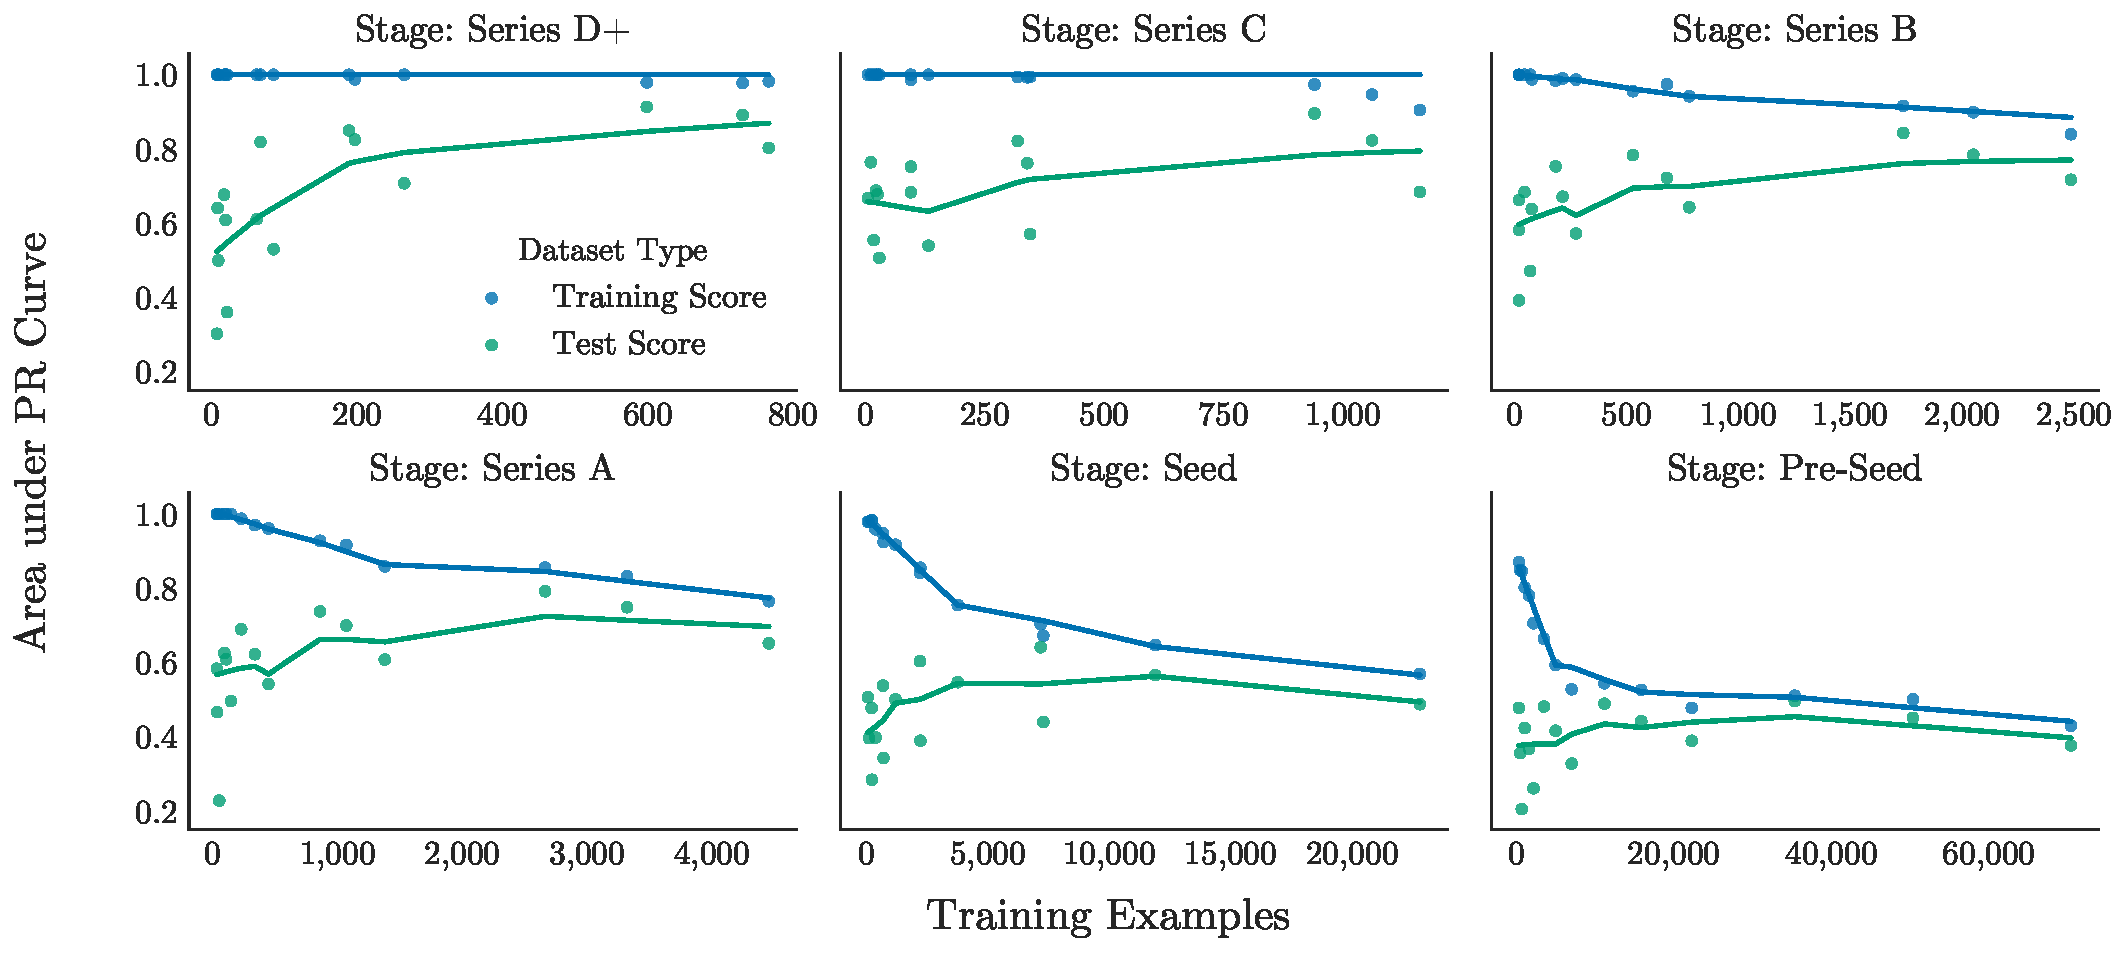
\includegraphics[width=\textwidth]{../figures/evaluation/learning_curves_stage}
    \caption[Learning curves by developmental stage]{Learning curves by developmental stage.}
    \label{fig:evaluation:learning_stage}
\end{figure}

\section{Versatility}

Our system must be consistently accurate at identifying a variety of high-potential investment candidates. We evaluated the systems' versatility based on its ability to predict over different forecast windows (e.g. 2--4 years), for target companies at different developmental stages (e.g. Seed, Series A, etc.), and for different target outcomes (e.g. predicting additional funding rounds, being acquired, having an \gls{ipo}, or some combination thereof).

\subsection{Forecast Window}

A forecast window is the period between when a prediction is made and when that prediction is evaluated (i.e. a prediction made in 2014 on whether a company would exit by 2017 is a forecast window of three years.) The \gls{vc} industry raises funds with fixed investment horizons (3--8 years)~\cite{gompers1995}, so time to payback is a key component of \gls{vc} investment decision-making and portfolio management. It is important we understand how the models and predictions produced by a \gls{vc} investment screening system vary with respect to the length of these forecast windows.

Figure~\ref{fig:evaluation:performance_window} shows model performance across a range of metrics, grouped by forecast window. We observe little difference in Area under the \gls{roc} curve across the forecast windows. However, across all three other metrics, there is a positive relationship between length of forecast window and model performance. The F1 Score shows the greatest improvement in performance over time (52.7\%), compared to Area under the \gls{pr} curve (34.1\%) and \gls{mcc} (11.6\%).

\begin{figure}[!htb]
    \centering
    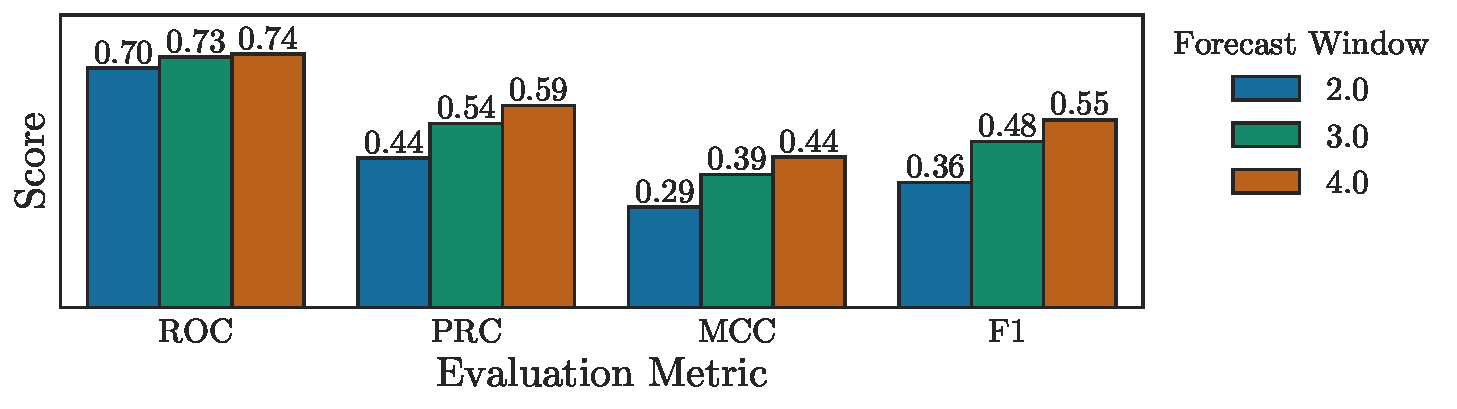
\includegraphics[width=\textwidth]{../figures/evaluation/performance_window}
    \caption[Performance by forecast window]{Performance by forecast window.}
    \label{fig:evaluation:performance_window}
\end{figure}

Figure~\ref{fig:evaluation:features_window} shows the standardised weights of features grouped using the conceptual framework proposed earlier in this paper, grouped by forecast window. First, we discuss the baseline distribution and then examine the variation in weightings with respect to forecast window. Factors related to advisors are the best predictor of startup investment success. Executives and founders features are also important factors and round out measures of human capital. The quality of investors that invest in a startup (assessed by their prior investments) is found to be more important than the quantum of investment raised by a startup. Local economy and industry features are weak predictors, as are customers and social influence (in this case, measured through participation at events). There is little difference between the weightings of each feature group with respect to forecast window. However, there are a few trends to point out: the importance of advisor factors increases over time, and the importance of executives and the broader economic factors decreases over time.

\begin{figure}[!htb]
    \centering
    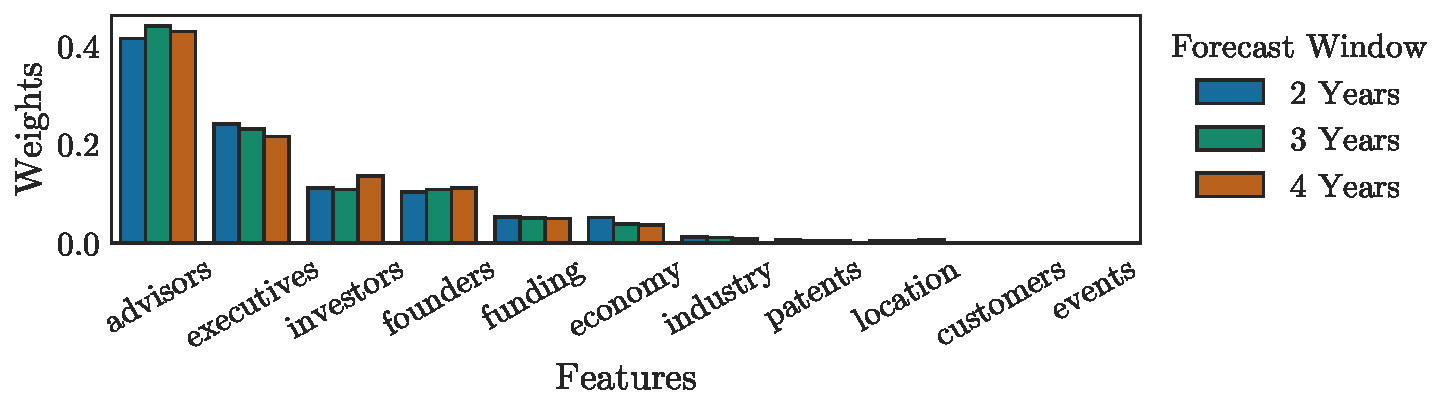
\includegraphics[width=\textwidth]{../figures/evaluation/features_window}
    \caption[Feature weights by forecast window]{Feature weights by forecast window.}
    \label{fig:evaluation:features_window}
\end{figure}

\subsection{Development Stage}

We can classify startups into developmental stages based on their external funding milestones. These milestones signal not only a change in the resources available to a startup, but also their functions and objectives, and in turn the type of investors that are interested in them as investment opportunities. In Chapter~\ref{chap:design} we mapped the companies in our dataset to their developmental stages. In the following section, we evaluated how the system models and predicts the outcomes of companies at different developmental stages.

Figure~\ref{fig:evaluation:performance_stage} shows F1 Scores grouped by developmental stage and fit method. First, we examined the baseline distribution and then the variation in performance by fit method. Model performance has a positive relationship with developmental stage. The only deviation from this relationship is for Series D+. To understand this discrepancy better, we split our datasets into their developmental stages and fit the model onto each of these sub-datasets individually (i.e. each dataset contains a single developmental stage). This method results in a broad performance improvement which has the least impact on Pre-Seed and the greatest impact on Series D+ companies.

\begin{figure}[!htb]
    \centering
    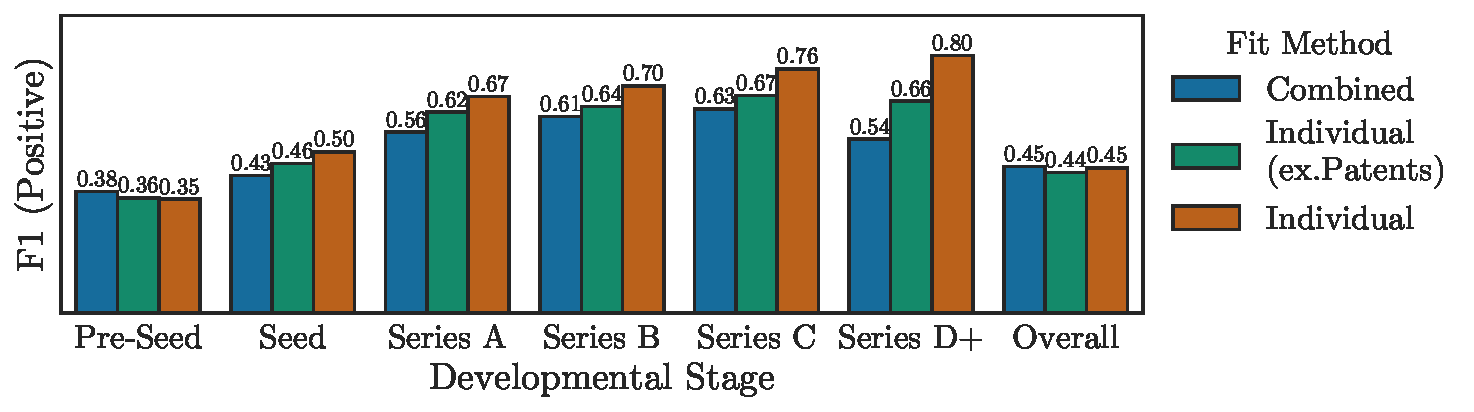
\includegraphics[width=\textwidth]{../figures/evaluation/performance_stage}
    \caption[Performance by developmental stage]{Performance by developmental stage.}
    \label{fig:evaluation:performance_stage}
\end{figure}

Figure~\ref{fig:evaluation:features_stage} shows the standardised weights of features, grouped by developmental stage. While we observe a similar trend to Figure~\ref{fig:evaluation:features_window}, there is more variation in weights than was seen when grouped by forecast window. Advisors are more important to earlier stage companies than late stage companies, investor track record and reputation becomes important as companies approach an exit (Series D+), executive and founder experience are important in pre-seed companies, as is broader economic outlook.

\begin{figure}[!htb]
    \centering
    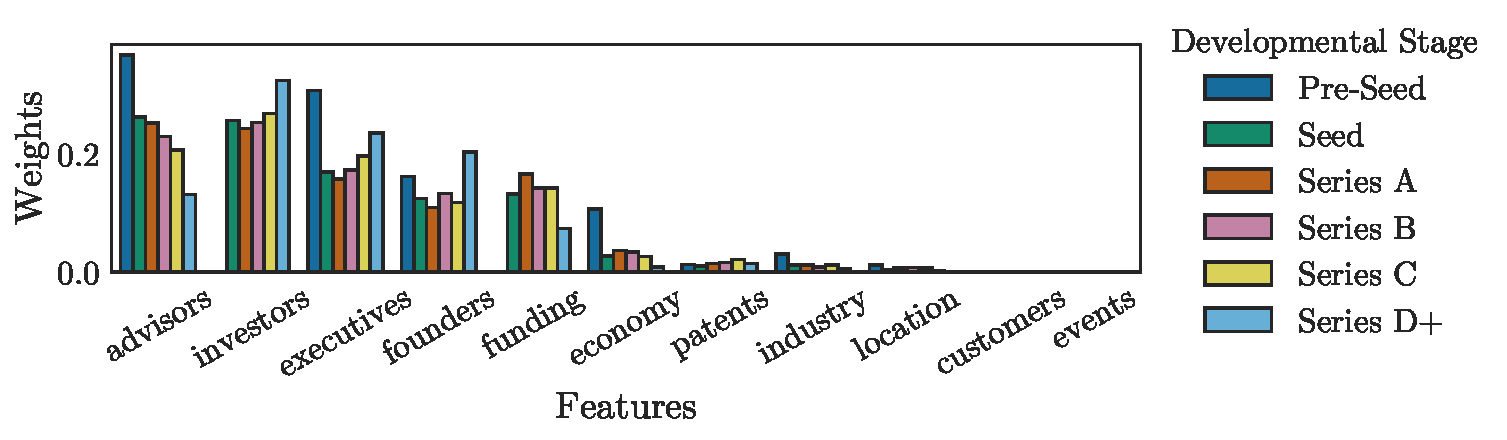
\includegraphics[width=\textwidth]{../figures/evaluation/features_stage}
    \caption[Feature weights by developmental stage]{Feature weights by developmental stage.}
    \label{fig:evaluation:features_stage}
\end{figure}

\subsection{Target Outcome}

Ultimately, \gls{vc} firms seek rare investments that will return their invested funds many times over within an investment horizon of their fund (3--8 years)~\cite{gompers1995}. Funds are only returned to \gls{vc} investors when startups have liquidity events (\gls{ipo}, Acquisition). However, recently, many companies that are considered successful are delaying their liquidity events and seeking later-stage private funding (e.g. Uber). In this case, whether a company has raised additional funding rounds may be used as a proxy for investment success. Unless otherwise specified, we performed our previous analyses against our base target outcome, Extra Stage (i.e. whether a company raises an additional funding round, is acquired or has an \gls{ipo}). In the following section, we explore whether other target outcomes have an effect on our system's predictive power.

Figure~\ref{fig:evaluation:performance_stage} shows F1 Scores grouped by target outcome and forecast window. First, we examine the baseline distribution and then the variation in performance by forecast window. Our model is most accurate at predicting extra funding rounds and worst at predicting IPOs. As we observed in Figure~\ref{fig:evaluation:performance_window}, there is a positive relationship between length of forecast window and model performance. This relationship has a similar magnitude across all target outcomes except for IPOs which improve more when we increase the forecast window from two to three years.

\begin{figure}[!htb]
    \centering
    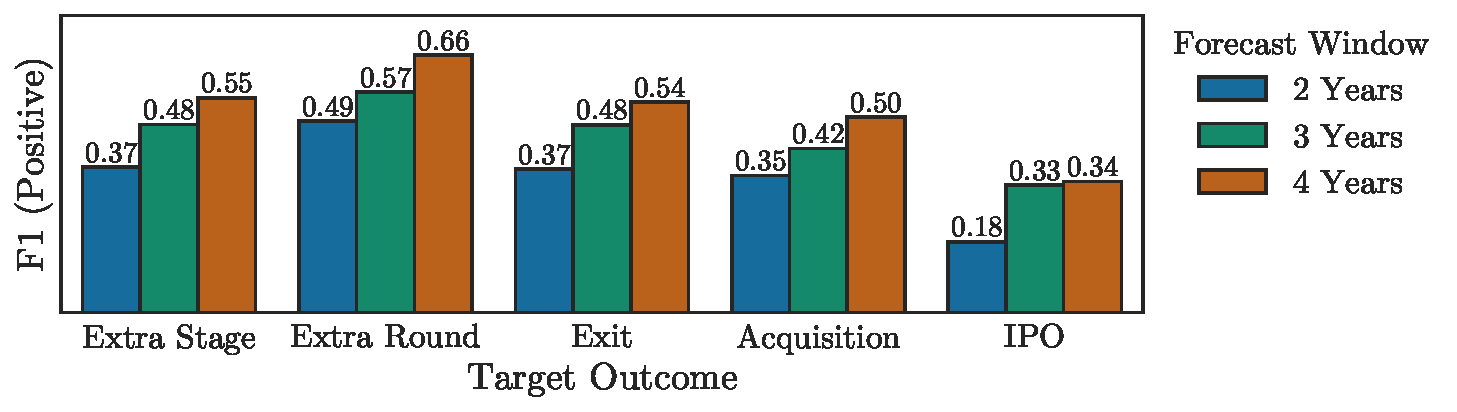
\includegraphics[width=\textwidth]{../figures/evaluation/performance_outcome}
    \caption[Performance by target outcome]{Performance by target outcome.}
    \label{fig:evaluation:f1_predictive_outcome}
\end{figure}

Figure~\ref{fig:evaluation:features_outcome} shows the standardised feature weight distribution, grouped by target outcome. Models of target outcomes produce considerable variance in feature weights. Exit and Acquisition have similar feature weights. Investors, Executives and Founders are key features for Exits and Acquisitions. In comparison, IPOs have greater weighting towards Funding, Advisors and the Broader Economy. Extra Round and Extra Stage have similar feature weights and are most strongly related to Advisors and Executives.

\begin{figure}[!htb]
    \centering
    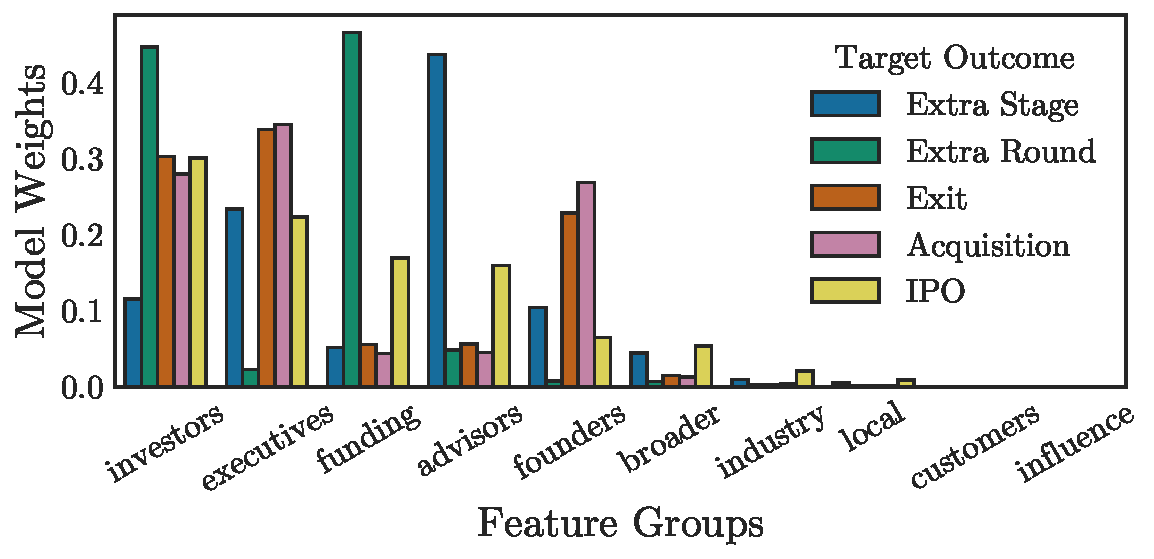
\includegraphics[width=\textwidth]{../figures/evaluation/features_outcome}
    \caption[Feature weights by target outcome]{Feature weights by target outcome.}
    \label{fig:evaluation:features_outcome}
\end{figure}

 \ifcsdef{mainfile}{}{\printbibliography}
\end{document}

